\RequirePackage{fixltx2e}[2005/12/01] 
\documentclass[useAMS,usenatbib]{mn2e}
\pdfoutput=1
\usepackage[varg]{txfonts}
\usepackage{astrojournals}
\usepackage{graphicx}
\usepackage{microtype}
\usepackage{xcolor}
\usepackage{hyperref}
\hypersetup{colorlinks=True, linkcolor=blue!50!black, citecolor=black,
  urlcolor=blue!50!black}

\begin{document}

\begin{figure}
  \centering
  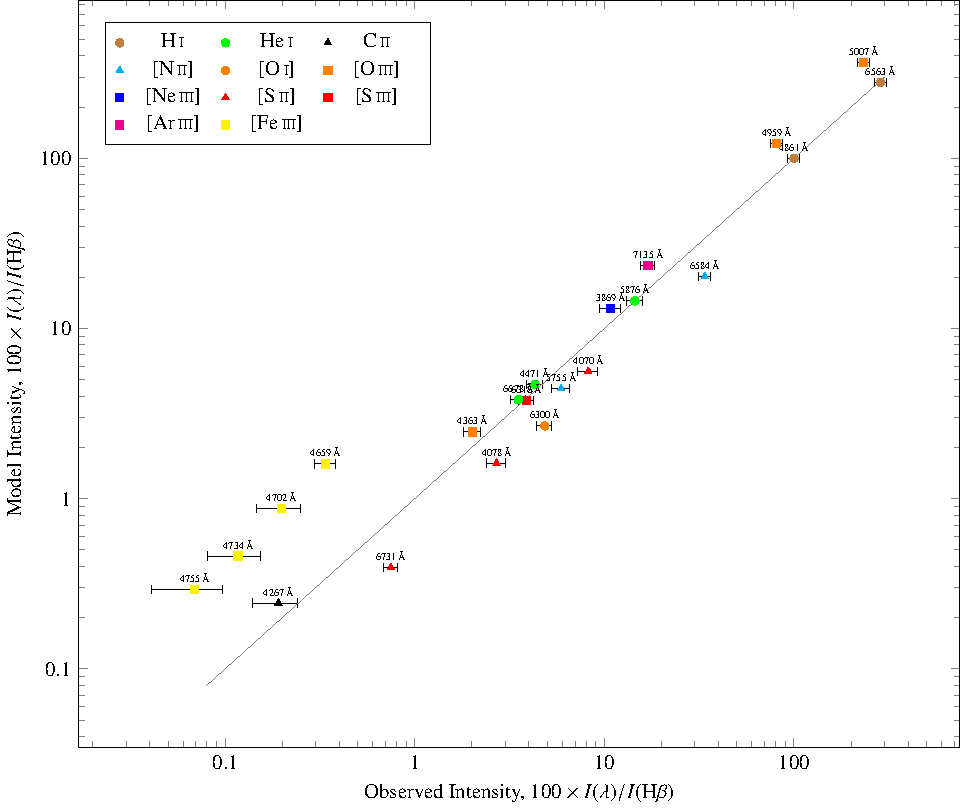
\includegraphics{ratios-figure-figure0}
  \caption{Comparison of model and observed line intensities for 177-341}
  \label{fig:model}
\end{figure}
\addtocounter{section}{6}
\addtocounter{subsection}{2}
\subsection{A physical model of 177-341}
As an alternative to the purely empirical analysis presented in the previous sections, a different approach to analysing the emission spectrum of the proplyds is through the construction of physical models that combine a priori simulations of radiative transfer, hydrodynamics, and atomic physics in order to predict the density, temperature, and ionization structure of the proplyd flow.  Such models have previously been applied to the ensemble properties of large numbers of proplyds 


\bibliography{BibdeskLibrary}

\end{document}
